\setcounter{chapter}{-1}
%\renewcommand{\chapter}[1]{\newchapter{#1}}


\newchapter[математического мышления]{Принципы}

\fancyhead[LE]{\hspace*{-15mm}\fcolorbox{darkred}{darkred}{%
\begin{minipage}{13mm}
\begin{flushleft}
\textcolor{white}{\phantom{\Large Y}\hspace*{-3mm}{\sffamily урок} \\[1mm] \bfseries\Huge\arabic{lektion}}
\end{flushleft}
\end{minipage}}}
\fancyhead[RO]{\hspace*{\textwidth}\fcolorbox{darkred}{darkred}{%
\begin{minipage}{13mm}
\begin{flushright}
\textcolor{white}{\phantom{\Large Y}{\sffamily урок}\hfill \\[1mm] \bfseries\Huge\arabic{lektion}}
\end{flushright}
\end{minipage}}}



\vrezka{В этой главе обсуждаются основные математические термины, способы суждений и доказательств, рассматриваются начала теории множеств.

Данная глава носит справочный характер и может быть пропущена при первом чтении конспекта.
}

\section{Символы и слова}

\lesson{Несколько терминов и обозначений. Пример построения фразы про крокодилов}
\href{https://www.youtube.com/watch?v=HbDwyaoG6mE}{Ссылка на видеоурок}

\begin{enumerate}
\item Фундаментальным понятием математики является \textbf{равенство} (=).\index{Равенство} Два объекта считаются равными, если они не отличаются по своим свойствам в рамках используемого языка. Можно привести пример с оттенками белого снега у народов Крайнего Севера. Они используют несколько десятков слов для обозначения оттенков белого цвета, в то время как для европейцев все эти оттенки в рамках разговорного языка равны, в нем нет обозначений такого количества оттенков белого (это не значит, что европеец не сумел бы физически отличить многие оттенки после длительной тренировки, просто ему это не нужно). Поэтому равенство, с одной стороны, относительно (есть имманентное свойство языка), а с другой стороны, фундаментально (как абстрактное понятие), т.к. лежит в основе всех математических утверждений, даже когда оно там не участвует явно.
\item Для более экономной записи сложных высказываний математики пользуются огромным количеством спецсимволов. Приведем расшифровку некоторых из них:

\begin{align*}
\forall & \quad\mbox{для любого} & \exists & \quad\mbox{существует}  \\
\cap & \quad\mbox{пересечение множеств} & \land & \quad\mbox{логическое И}  \\
\cup & \quad\mbox{объединение множеств} & \lor & \quad\mbox{логическое ИЛИ}  \\
\setminus & \quad\mbox{разность множеств} & \neg & \quad\mbox{логическое НЕ}  \\
\in & \quad\mbox{принадлежит} & \subseteq & \quad\mbox{содержится}  \\
\emptyset & \quad\mbox{пустое множество} & \vdash & \quad\mbox{противоречие/выводимость}
\end{align*}

\item Пусть $K$ --- множество всех крокодилов, $M$ --- множество всех животных в Москве-реке, а свойство $c(k)$ обозначает цвет объекта $k$. Высказывание
$$
\forall k\in K\cap M\;c(k)= {}'\mbox{красный}'
$$
переводится следующим образом: все крокодилы в Москве-реке красные. Кстати оно является истинным, т.к. его невозможно опровергнуть, ведь в Москве-реке не водятся крокодилы.

\item Помимо специальной символики математики постоянно жонглируют профессиональной терминологией. Многие, известные со школы, понятия, имеют непривычные обывателю названия. Приведем несколько примеров для сравнения:
\begin{center}
\begin{tabular}{r|l}
переместительный закон & коммутативность \\
сочетательный закон & ассоциативность \\
распределетильный закон & дистрибутивность
\end{tabular}
\end{center}

Напомним, что переместительный закон сложения означает, что
$$
a+b = b+a.
$$
Сочетательный закон сложения означает, что
$$
a+(b+c) = (a+b)+c.
$$
А распределительный закон связывает сложение и умножение по правилу:
$$
a(b+c) = ab + ac.
$$

\item Стоит отдельно сказать пару слов и о термине «рациональный». В математике обыкновенная дробь $m/n$ (где число $m$ является целым, а число $n$ --- натуральным) называется рациональным числом. Соответственно, всякое число, которое не является рациональным, называется <<иррациональным>> (речь идет о числах на числовой оси). Такие числа были открыты еще пифагорейцами.

Слово «иррациональный» в обычной жизни имеет отрицательную коннотацию, хотя в математике это всего лишь отрицание рациональности, и никак не связано со знаком <<минус>> перед числом.

Заметим, что многие математические термины, на самом деле, имеют греко-латинское происхождение (как и вообще многие научные термины), но в школьной программе они были переведены на русский язык, а затем закрепились за частным случаем своего греко-римского аналога --- их стали относить только к операциям с числами и векторами, в то время как исходные научные термины имеют более широкую область применения.

\item <<Трансцендентность>> в философии означает то, что находится за гранью логического восприятия, а в математике число трансцендентно, если оно не является алгебраическим (т.е. корнем многочлена) над конкретным полем. То есть в математике это еще и относительное понятие, хотя чаще всего подразумевается трансцендетность относительно множества рациональных чисел.
\item Приведем шуточный, но вполне строгий пример математического рассуждения. Три математика приходят в бар, садятся за столик, и подошедший официант задает им вопрос:

--- Все будут пиво?

--- Не знаю, --- отвечает первый математик, подумав.

--- Не знаю, --- отвечает второй математик.

--- Все! --- отвечает третий.


Почему они все отвечали именно так? Первый не знал, чего хотят остальные, но сам хотел пива, поэтому ответил «не знаю». Если бы он не хотел, то сразу бы ответил «нет», т.к. уже было бы понятно, что не все хотят пиво (ведь «не все хотят», значит, «хотя бы один не хочет»). Второй после ответа первого уже понял, что первый будет пиво, но не знал про третьего, а сам тоже хотел. Поэтому тоже ответил «не знаю». Наконец, третий математик из их ответов понял, что они хотят пиво (иначе бы кто-то из них или оба ответили бы «нет»), сам он тоже хотел, так что можно было смело сделать вывод, что пиво будут все, поэтому на вопрос официанта он ответил «все!».

\item Еще один простой пример: кого больше --- львов или зверей? Здесь ответ кроется в том, что всякий лев есть зверь, но не всякий зверь есть лев, так что зверей явно больше (если, конечно, тех и других не бесконечно много, но мы живем в мире, где даже атомов --- конечное число, а уж тем более львов, зверей и живых существ).

\item Выше мы вводили произвольные обозначения для множества крокодилов и множества зверей, поскольку в математике нет устоявшегося обозначения для них. А одно множество было нами обозначено символом $\emptyset$. Это --- стандартное обозначение множества, не содержащего элементов, т.е. пустого. По-другому его еще обозначают скобками без содержимого: $\{\}$.

Есть, однако, ряд стандартных символов для обозначения некоторых конкретных непустых множеств. Речь идет о следующих обозначениях:
\begin{align*}
\N=\{0,1,2,3,\dots\} & \quad\mbox{множество натуральных чисел} \\
\Z=\{0,\pm1,\pm2,\pm3,\dots\} & \quad\mbox{множество целых чисел} \\
\Q=\{m/n\mid m\in\Z, n\in\N, n\ne 0 \} & \quad\mbox{множество рациональных чисел (дробей)} \\
\R & \quad\mbox{множество действительных чисел} \\
\C & \quad\mbox{множество компл\'eксных чисел}
\end{align*}
\end{enumerate}

\section{Математические рассуждения}

\lesson{Примеры суждений, непривычных для бытовой логики: про голосование, про хлеб и т.д.}
\href{https://www.youtube.com/watch?v=Tr5E_FZaMh4}{Ссылка на видеоурок}

\begin{enumerate}
\item \textbf{Особенности языка}. Так же, как равенство является неотъемлемым понятием языка (кроме некоторых совсем уж бедных искусственных языков), сам язык является довольно точным отражением мышления его носителей и, главное, области своего применения. В тех областях знаний, где точность играет если не первую, то уж точно не последнюю роль, мышление специалистов накладывает некоторые (порой весьма причудливые) ограничения на язык, которым они пользуются при написании высказываний, суждений, догматов и предписаний. Чем более беспристрастно и точно требуется выразить мысль, тем более странным может показаться язык, которым она записана.

Это явление редукции живого разговорного языка до некоторого канцелярского варианта, в котором значения терминов определяются максимально строго, А.~П.~Ершов назвал <<деловой прозой>>. К деловой прозе относятся естественнонаучные, математические, юридические тексты, тексты делопроизводства (т.е. собственно канцелярские), инструкции и т.п. Само собой, язык деловой прозы требует специального обучения. Это особенно важно для правильного понимания инструкций. Их понимание может вызывать проблемы.

Приведем одну из таких проблем, случившихся на практике. Чтобы стать членом некоего общества гуманитарной направленности, надо пройти процедуру голосования на имеющиеся вакансии. Правом голоса обладают все члены общества, голосование проводится турами. Положение о выборах было написано
математиками. Оно гласит:\footnote{Здесь мы цитируем книгу Успенского \cite{Usp0}.}

\textit{Для избрания членом общества необходимо получить
не менее $2/3$ голосов лиц, принявших участие в голосовании, и не менее половины от списочного состава
общества. Кандидат считается избранным в данном туре
голосования, если в этом туре он получил необходимое
для избрания число голосов и число всех кандидатов,
получивших в этом туре такое же или большее число
голосов, не превышает числа вакансий по данной специальности, оставшихся незаполненными в предыдущих
турах (в первом туре --- числа всех имеющихся вакансий). Если в первом туре голосования число избранных
кандидатов по данной специальности оказалось меньше,
чем число вакансий по этой специальности, то проводится второй тур голосования. Если по результатам первого
и второго туров остались незаполненные вакансии по
данной специальности, то проводится третий тур голосования.
}

Случилось так, что при выборах на единственную вакансию
каждый из кандидатов $X$ и $Y$ получил во втором туре не менее
$2/3$ голосов лиц, принявших участие в голосовании, и не менее
половины списочного состава. При этом $Y$ получил больше голосов, чем $X$. Два вопроса: избран ли кто-нибудь в этом туре, и если
избран, то кто? надо ли проводить третий тур? Эксперимент показал, что математики отвечают на этот вопрос, как правило,
верно, тогда как гуманитарии, как правило, неверно. Верные ответы состоят в том, что $X$ не избран, избран $Y$ и что третий тур
проводить не надо. Это обосновывается следующим рассуждением. Имеются два условия избрания. Первое условие --- получить
необходимое количество голосов: не менее $2/3$ голосов участвующих в голосовании и не менее половины от списочного состава. Второе условие --- количество $N$ всех кандидатов, получивших
в этом туре такое же или большее число голосов, не превышает
числа $P$ вакансий. В нашем примере первое условие выполнено
для обоих кандидатов. Посмотрим, что происходит со вторым
условием. В нашем примере число вакансий $P$ равно $1$. Для $X$ второе условие не выполнено, поскольку для этого кандидата $N = 2$
и тем самым $N$ превышает $P$. Для $Y$ второе условие выполнено,
поскольку для этого кандидата $N = 1$ и тем самым $N$ не превышает $P$. В реальности же был проведён третий тур, в котором
избранным оказался $X$.

\item \textbf{Внимание к деталям}. В том случае, когда математик сталкивается с неродным ему языком, он непроизвольно ищет способ строго выразить сказанное или написанное так, чтобы не возникало разночтений, для чего, как правило, приходится привлекать некоторый формальный аппарат.

Рассмотрим две задачи-вопроса. Самый старший математик среди шахматистов и самый старший шахматист среди математиков --- один и тот же человек? А самый крутой математик среди шахматистов и самый крутой шахматист среди математиков --- один и тот же человек? (эти задачи взяты из книги Верещагина и Шеня \cite{Vereschagin})

Здесь первое, что нужно уточнить --- какова природа метрики, по которой мы сравниваем объекты. В первом случае это возраст. Данная метрика является универсальной для всех людей, в частности, для класса математиков и класса шахматистов она \textit{одна и та же}. Иначе говоря, мы сравниваем два множества объектов по одной и той же шкале. И поскольку математики, являющиеся шахматистами, и шахматисты, являющиеся математиками, --- суть одни и те же люди, то и максимум по возрасту у них будет один и тот же. Таким образом, в первом вопросе ответ --- да, один и тот же.

Второй вопрос сложен тем, что метрика <<крутости>> не является универсальной, т.е. в классе математиков и в классе шахматистов она определяется по-своему (выявлению этого факта способствует неявное указание на тип измеряемого по крутости объекта --- математик или шахматист). А это значит, что максимум по метрике <<крутости>> в классе математиков-шахматистов зависит от конкретизации этой метрики: привязана ли она к умению играть в шахматы или к умению получать математические результаты. Поэтому ответ на второй вопрос --- нет, не обязательно один и тот же.

Подчеркнем, что в данном сюжете мы использовали слово метрика не в математическом смысле. В математике метрика --- это расстояние между двумя точками. А <<крутость>> или возраст --- это, скорее, мера.

\item \textbf{Ложная посылка}. Рассмотрим теперь некое суждение, имеющее логический конструкт \textit{импликации} $x\to y$ (из $x$ следует $y$):
\begin{center}
(A)\quad Если Земля плоская, то все крокодилы красные.
\end{center}
Поскольку мы придерживаемся общепринятой логики и соблюдаем закон Tertium non datur (третьего не дано), истинным может быть либо само это высказывание, либо его отрицание. Отметим, что отрицанием данной импликации (A) является следующее высказывание:
\begin{center}
(B)\quad Земля плоская И крокодилы НЕ красные.
\end{center}
Итак, высказывание (B) есть отрицание высказывания (A).

Поскольку мы знаем, что Земля не плоская (а это знал еще Эратосфен Киренский, который довольно точно измерил ее радиус в 3 веке до н.э.), высказывание (B) ложное (здесь уже не важно, какой цвет у крокодилов, т.к. в высказывании с союзом И достаточно одной части быть ложной, чтобы все высказывание стало таковым же). Но тогда высказывание (A) истинное!
Несмотря на то, что посылка высказывания (A), которая утверждает, что Земля плоская, ложна.

Иначе говоря, из ложной посылки следует любое высказывание --- хоть истинное, хоть ложное. Также и истинное высказывание следует из любой посылки --- хоть истинной, хоть ложной.

Подчеркнем, что отличием математической логики от обычной, причинно-следственной, является то, что мы не увязываем посылку и следствие какой-то смысловой связью, а смотрим только на их истиность или ложность в контексте данной теории. Тем не менее, нужно заметить, что построение выводов при доказательстве теорем почти всегда имеет осмысленную причинно-следственную связь, т.к. только таким способом можно нащупать истинную импликацию.

\item \textbf{Элементарные рассуждения}. Рассмотрим арифметический пример высказывания:
\begin{center}
(C)\quad Если $a$ --- четное число, то оно делится на 4.
\end{center}
Такое высказывание ложно, т.к. не все четные числа делятся на 4. Обратно,
\begin{center}
(D) если число делится на 4, то оно четное.
\end{center}
А это высказывание уже истинное.

Высказывание (D) является \textit{дедуктивным}, поскольку основано на строгом выводе из свойств натуральных чисел. Оно \textbf{выводится} из аксиом или ранее доказанных теорем.

Высказывание (C) может быть лишь предположением. Если бы мы взяли числа $4,16,32,64,128,256,512,1024$, то оказалось бы, что все они не только четные, но и делятся на 4. Может возникнуть подозрение, что так бывает всегда, и мы строим гипотезу: если число четное, то оно делится на 4. Но затем мы обнаруживаем, что, например, 6 не делится на 4, хотя является четным (т.е., как говорят математики, мы нашли \textbf{контрпример}). Гипотеза оказывается неверной.

Высказывания-гипотезы, которые строятся на основе наблюдений и опыта, могут быть индуктивными и абдуктивными. К \textbf{индуктивным} относят такие суждения, когда был произведен довольно длительный ряд наблюдений в одних и тех же условиях, и всегда выполнялось одно и то же измеряемое свойство (например, сколько мы ни брали нечетных чисел, а их квадрат всегда имел вид $4k+1$). Тогда мы строим гипотезу, что это свойство верно всегда в подобных ситуациях (в нашем примере --- предполагаем, что у любого нечетного числа квадрат имеет вид $4k+1$).

Вышеупомянутая гипотеза (C) может бы получена индукцией, если основываться на данных ряда $4,16,32,64,128,256,512,1024$.

Предположим, что в таком же опыте (длительная серия наблюдений в одних и тех же условиях) измеряемое свойство наблюдалось не всегда, но с какой-то регулярностью. Например, мы брали все числа подряд и возводили в квадрат, и в каких-то случаях получали число вида $4k+1$, в каких-то --- нет. Далее мы смотрим на эту серию наблюдений и пробуем понять, какой вид имеет число, квадрат которого имеет вид $4k+1$. Например, мы можем предположить что оно простое (ведь для всех простых, кроме двойки, это верно), или же, что оно нечетное. Ясно, что нечетных чисел в выборке окажется сильно больше, чем простых, так что мы склонны будем сформулировать гипотезу о том, что если квадрат числа имеет вид $4k+1$, то это число --- нечетное.

Гипотеза, в которой по наблюдаемому следствию выбирается причина (обычно --- наиболее вероятная, если их несколько), называется \textbf{абдуктивной}. На основе адуктивной гипотезы (как и индуктивной) можно сформулировать теорему и попытаться ее доказать (либо найти контрпример).

Похожие рассуждения имеют место при использовании метода максимального правдоподобия при построении гипотез и оценок в статистике, а также в машинном обучении и искусственном интеллекте. Такими же рассуждениями мы пользуемся повседневно, относя их к жизненному опыту. На таком же методе, в основном, был построен знаменитый метод рассуждений Шерлока Холмса, который ошибочно называют дедуктивным.

\item \textbf{Недопонимание}. Привычка математиков сводить высказывания к строгому языку, отстраняясь от конкретного контекста и его внутренней логики, приводит порой к неожиданным и анекдотическим последствиям. Вот один характерный пример-анекдот.

Жена просит мужа-математика <<Купи батон хлеба, а если будут яйца, то купи десяток>>. Он приносит 10 батонов хлеба. (Поскольку жена не уточняет, десяток чего именно надо купить, муж использует тот же контекст, который вначале соответствует глаголу <<купить>>, а наличие яиц в магазине воспринимает как внешнее дополнительное условие.)
\end{enumerate}


\section{Функции}

\lesson{Примеры функций, функция как отношение, обратная функция}
\href{https://www.youtube.com/watch?v=KiOvT74eXw0}{Ссылка на видеоурок}

Более подробный материал см. в разделах \ref{Rels} и \ref{functions}

\begin{enumerate}
\item Пусть есть два множества $A$ и $B$ произвольной природы. \textbf{Прямым произведением} этих множеств называется множество всех упорядоченных пар вида $(a,b)$, где $a\in A, b\in B$. Прямое произведение обозначается $A\times B$. В общем случае $A\times B\ne B\times A$.
\item Функцией из $A$ в $B$ называется подмножество $f\subseteq A\times B$ такое, что если $(a,b)\in f$ и $(a,c)\in f$, то $b=c$, и кроме того, для всякого $a\in A$ найдется $b\in B$ такое, что $(a,b)\in f$.
\item Функция задает однозначное соответствие элементов множества $A$ элементам множества $B$.
\item Обозначения. Функция: $f:A\to B$. Значение функции: $b=f(a)$.
\item Например, пусть $b=f(a)$ означает, что $b$ есть отец $a$. Функция $f$ в данном случае определена на множестве людей и принимает значения там же. Поскольку у каждого человека отец ровно один, это --- функция.
\item Над функциями существует операция композиции, если одна функция принимат значения в области определения другой. Пусть $f:A\to B$ и $g:B\to C$. Тогда можно определить функцию $h=g\circ f$, которая работает следующим образом: 
$$
h(a) = g(f(a)),
$$
и является функцией вида $h:A\to C$. Иначе говоря, запись $g\circ f$ обозначает последовательное применение функций в порядке справа налево, что соответствует порядку записи функций в выражении $g(f(a))$. Если функции действуют на одном множестве, то на них автоматически задана операция композиции, которая, к тому же, является ассоциативной: $h\circ (g\circ f)=(h\circ g)\circ f$.
\item Если мы обозначим через $g(a)$ деда человека $a$, то это уже не функция, а отношение, т.к. у каждого человека два деда.
\item Если мы будем каждому человеку ставить в соответствие набор его паспортных данных (серию и номер, место рождения, дату рождения, полное ФИО), то этот набор будет однозначно определять человека. И тут функция станет обратимой: по паспортным данным можно вычислить человека.
\item В связи с этим различают следующие виды функций:

\textbf{Сюръекция}: функция $f:A\to B$, значениями которой являются все элементы множеста $B$. При этом она может принимать одно и то же значение в разных точках множества $A$.\index{Функция!сюръекция}

\textbf{Инъекция}: функция $f:A\to B$, которая в разных точках множества $A$ принимает разные значения из множества $B$. При этом не требуется, чтобы она принимала все значения из множества $B$.\index{Функция!инъекция}

\textbf{Биекция}: функция, которая является одновременно сюръекцией и инъекцией. Биекция $f:A\to B$ осуществляет взаимно однозначное соответствие всех точкек множества $A$ всем точкам множества $B$.\index{Функция!биекция}

\item \textbf{Отношение между множествами} $A$ и $B$ есть подмножество в прямом произведении $A\times B$. Если $A=B$, то отношение $R\subseteq A\times A$ называется \textbf{отношением на множестве} $A$.

Например, можно рассмотреть отношение дружбы на множесте всех людей.

Отношения бывают разных видов: симметричные, рефлексивные, транзитивные, эквивалентности, линейного порядка и т.д. Подробнее эти виды отношений мы рассмотрим в разделе \ref{Rels}.

Функция --- это также разновидность отношения. Причем функция является отношения <<многих к одному>> или <<один к одному>> (многие дети к одному отцу), а произвольное отношение может быть также отношением <<многих ко многим>> (дружба) или одного ко многим (отец ко многим детям, внук к двум дедам).

\item Отношение $R\subseteq A\times B$ можно развернуть, т.е. построить отношение на множестве $B\times A$, взяв вместо пар $(a,b)$ пары $(b,a)$, т.е. записать их в обратном порядке. Такое отношение называется \textbf{обратным} к исходному и обозначается $R^{-1}$.

\item Если отношение $F$ --- функция, и отношение $F^{-1}$ --- функция, то $F^{-1}$ называется \textbf{обратной функцией} к функции $F$. Всякая биекция обратима, и обратная к биекции функция также является биекцией. Кроме того, $(F^{-1})^{-1}=F$, если $F$ обратима.

\end{enumerate}


\subsection*{Задачи}

\begin{enumerate}
\item Пусть $f$ --- функция <<отец>>, как определено выше. Запишите функцию <<дед по отцу>> с помощью $f$ и символа композиции функций.
\end{enumerate}



\section{Методы доказательств}

\lesson{Примеры использования принципа Дирихле, метода бесконечного спуска, индукции, контрапозиции, перебора, инварианта}
\href{https://www.youtube.com/watch?v=vjJwmACdD_U}{Ссылка на видеоурок}

Здесь мы приводим ряд примеров математических задач, демонстрирующщих основные математические методы.

\begin{enumerate}
\item \textbf{Принцип Дирихле}. Доказать, что среди произвольных $n$ натуральных чисел найдется несколько подряд идущих, сумма которых делится на $n$.

Принцип Дирихле заключается в следующем: если у вас имеется $K$ ящиков и $n$ шариков, разложенных произвольно по этим ящикам,  причем $n>K$, то хотя бы в одном ящике окажется хотя бы 2 шарика. Это утверждение вполне очевидно, т.к. если бы в каждом ящике было бы не более чем по одному шарику, то шариков было бы не более $K$. Посмотрим, как это работает в описанной задаче.

Пусть даны $a_1,\dots,a_n$ --- произвольные натуральные числа (не обязательно все различные). Рассмотрим накопленные суммы
$$
b_0=0, b_1=a_1, b_2=a_1+a_2,\dots, b_n=a_1+\dots+a_n.
$$
Получаем $n+1$ натуральное число (опять же, некоторые могут совпадать, если в исходной последовательности были нули). Вопрос: какие могут быть остатки от деления на $n$ у этих накопленных сумм? Очевидно, что остатками могут быть только числа $0,1,\dots n-1$, т.е. не более чем $n$ разных остатков. Но чисел у нас $n+1$, следовательно, в силу принципа Дирихле найдется два числа $b_k$ и $b_j$ с несовпадающими номерами $k\ne j$, остатки у которых совпадут (остатки --- это те самые ящики). Для определенности будем считать, что $k<j$ (в противном случае переобозначим).

Итак, $b_k=tn+r$ и $b_j=sn+r$, откуда получаем, что $b_j-b_k=(s-t)n$, т.е. данная разность делится на $n$. Но эта разность и есть сумма подряд идущих исходных чисел:
$$
b_j-b_k=a_j+a_{j-1}+\dots+a_{k+1}.
$$


\item \textbf{Метод бесконечного спуска}. Задача про черта и бизнесмена: бизнесмен отдает черту купюру, а взамен получает сколько угодно купюр меньшего достоинства, либо ничего не получает, если таких купюр не существует. Доказать, что за конечное число шагов бизнесмен разорится.

Здесь нужно следить за величиной, равной максимальному номиналу среди всех купюр бизнесмена. Бизнесмен может начинать размен с любой купюры, пусть даже самого малого достоинства (не получая взамен ничего).

Ясно, во-первых, что эта величина не может возрастать, поскольку всякий размен либо сохраняет ее (еще остаются купюры данного номинала), либо уменьшает (когда была разменена последняя купюра максимального номинала).

Предположим теперь, что бизнесмен играет таким образом, что количество купюр максимального номинала не уменьшается, т.е. остается постоянным. В этом случае мы можем вообще забыть про эти купюры и рассматривать игру тлько с купюрами меньшего достоинства. Рассмотрим следующий по величине номинал среди его купюр. Очевидно, что при такой игре количество купюр следующего по величине номинала не может расти (по тем же соображениям, ведь для роста их количества требовалось бы уменьшить количество купюр старшего номинала, а мы договорились их не трогать). Тем самым мы воспроизводим предудщую ситуацию, но с меньшим максимальным номиналом.

Предположим снова, что бизнесмен играет так, что и количество вторых по величине купюр не убваает, т.е. остается постоянным. Тогда мы можем забыть и про них, и рассматривать задачу только с купюрами еще более мелкого достоинства.

Рассуждая аналогичным способом, мы можем бесконечно понижать достоинство старших купюр в игре. И вроде бы все у бизнесмена будет хорошо. если бы не одно НО: количество различных достоинств купюр ограничено! Рано или поздно наш бесконечный спуск по номиналам купюр упрется в самый маленький номинал среди всех имеющихся у бизнесмена. И в этом случае для продолжения игры ему придется снизить количество купюр данного номинала. При этом, правда, у него могут появиться купюры еще более низкого достоинства (если их еще не было), но и такой переход рано или поздно упрется в тот факт, что купюр еще более мелкого номинала, чем есть в данный момент у бизнесмена, просто не существует. И наш бесконечный спуск окажется конечным.

Таким образом, невозможно заморозить количество купюр самого мелкого достоинства, откуда следует, что невозможно заморозить количество купюр предыдущего достоинства, откуда следует, что невозможно заморозить количество купюр еще более высокого достоинства, и т.д. А раз у нас изначально было конечное количество различных номиналов, то и количество купюр максимального номинала невозможно сохранять постоянным. Оно неизбежно будет убывать на некоторм шаге игры.

Отсюда уже следует, что рано или поздно (поскольку число купюр конечно) купюры максимального достоинства закончатся. и мы перейдем к игре с меньшим номиналом. И так далее, пока не останутся купюры только самого маленького из возможных номиналов, и бизнесмен будет вынужден отдать их всех, ничего не получая взамен.

В решении данной задачи мы использовали еще один метод (наверное, самый популярный) --- метод \textbf{<<рассуждения от противного>>}. Мы предполагали, что количество купюр определенного номинала можно оставить постоянным (не уменьшать) и пришли к противоречию уже с помощью метода бесконечного спуска.

\item \textbf{Перебор вариантов}. Некоторые задачи решаются только перебором вариантов. При этом нужно уметь максимально сузить список вариантов и показать, что он исчерпывает все возможные ситуации. Далее остается пройтись по этому списку и показать возможность или невозможность решения задачи, тем самым, предъявляя алгоритм решения. Некоторые очень сложные задачи сводятся к компьютерному перебору многих тысяч вариантов. Но если строго показано, что других вариантов быть не может, а во всех имеющихся получен (или посчитан на компьютере) тот или иной ответ, то задача решена.

Рассмотрим такую задачу: 9 монет, одна фальшивая, причем известно, что она тяжелее остальных. Сколько нужно взвешиваний на весах с двумя чашами, чтобы найти фальшивку? 

Задача решается построением алгоритма последовательного уменьшения множества монет, содержащих фальшивую монету. Поскольку у весов 2 чаши, мы будем двигаться вниз постоянным делением множества монет на 3 равные части.

Итак, $9=3+3+3$. Взвесим 3 монеты, выбранные наугад, против других 3 монет, выбранных наугад. Если весы в равновесии, то фальшивая монета --- среди тех трех, что не на весах. Если же весы не в равновесии, то фальшивая монета в более тяжелой чаше, где также 3 монеты. Таким образом, мы нашли множество из 3 монет, среди которых одна фальшивая.

Далее, поскольку $3=1+1+1$, взвесим любые две из них. Если весы в равновесии. то фальшивая монета --- та, что не на весах. Если же весы не в равновесии, то фальшивая --- та, что тяжелее. Итак, всего 2 взвешивания!

Чтобы доказать, что задача, вообще говоря, не решается за 1 взвешивание, заметим, что как бы мы ни делили множество из 9 монет на 3 группы, всегда будет множество, содержащее более 1 монеты, в котором как раз и может оказаться фальшивая.

Тем не менее, кому-то может повезти, если он взвесит две кучки монет по 4 штуки в каждой, и весы останутся в равновесии, в этом случае фальшивая монета обнаружится за 1 шаг. Но если весы не окажутся в равновесии, то потребуется еще 1 или 2 взвешивания до получения результата.

Здесь проявляется такой интересный момент при работе с математикой, когда мы требуем минимизировать количество взвешиваний и находим алгоритм, который справляется точно за 2 взвешивания, и точно за 1 взвешивание не справляется. В то же время, задачу можно интерпретировать чуть иначе, и дать такой ответ: от 1 до 3 взвешиваний. Если вам повезет, то вы можете воспользоваться вторым способом и сразу найти фальшивку, но если не повезет, то второй метод может дать и два, и три шага. Поэтому настоящее математическое исследование вопроса предполагает рассмотрение всевозможных путей решения задачи с описанием их достоинств и недостатков. В частности, можно заявить, что с вероятностью 1/9 можно определить фальшивку за 1 шаг, но если не повезло, то дальше с равными шансами останется еще 1 или 2 взвешивания (поскольку подозрительными будут 4 монеты).

\item \textbf{Инвариант}. В квадрате $8\times 8$ клеток вырезали две угловых клетки в противоположных углах. Можно ли полученную фигуру замостить доминошками $1\times 2$?

Здесь используется метод инварианта. Инвариант --- это некоторая величина, которая не меняется при действиях, разрешенных правилами задачи (игры).

В данном случае действиями являются различные способы выкладывания доминошек на доску. А инвариант вводится искусственно с помощью дополнительной раскраски доски.

Итак, закрасим доску в шахматном порядке черными и белыми клетками, тогда клеток одного цвета будет на 2 меньше, чем другого. Но доминошки, как бы мы их не выкладывали на доску, всегда закрывают 1 белую клетку и 1 черную, поэтому разность между количеством закрытых белых клеток и количеством закрытых черных клеток всегда равна нулю. Если бы требуемое замощение существовало, то на доске без вырезанных углов было равное количество черных и белых клеток, а это не так. Следовательно, такое замощение невозможно.

Эта задача демонстрирует нам тот тип математических результатов, которые с трудом даются неподготовленному человеку. В таких задачах мы строго доказываем, что какой-то конструкции не может быть в принципе. При этом мы не перебираем все триллионы триллионов вариантов размещений доминошек (что в принципе невозможно физически), а пользуемся простыми логическими соображениями.

\end{enumerate}



\section{*Канторова теория множеств}

\lesson{Рассуждения о бесконечных множествах, равномощность $\N$ и $\Q$. Теорема Кантора}
\href{https://www.youtube.com/watch?v=9PlZC2mFNeQ}{Ссылка на видеоурок}

Более подробно см. раздел \ref{powers}

\hard{
\begin{enumerate}
\item Множества \textbf{равномощны}, если между ними существует взаимно однозначное соответствие.
\item Конечное множество характерисзуется тем, что никакая его собственная часть не равномощна всему множеству. С бесконечными все как раз наоборот.
\item <<Отель Гильберта>>.
\item Равномощность натурального ряда и множества целых чисел: четным числам ставим в соответствие положительные, нечетным --- отрицательные, нулю --- ноль.
\item Теорема Кантора: никакое множество не равномощно множеству всех своих подмножеств.
\end{enumerate}
}

\quad











\begin{comment}

\newchapter{Логика и мнжества (факультативно)}

\vrezka{В этой главе обсуждаются основы математической логики и теории множеств, построение высказываний и множеств на бытовых примерах. Вводится понятие суммы и произведения числовых множеств по Минковскому.

Данная глава носит справочный характер и может быть пропущена при первом чтении конспекта. Тем не менее, настоятельно рекомендуется регулярно возвращаться к ней по мере освоения материала.
}



\section{Суждения и силлогизмы}


\subsection*{Конспект}
\begin{enumerate}\setlength{\itemsep}{1pt}
\item Типовая конструкция суждения: \textbf{Посылки} $\vdash$ \textbf{Вывод}.
\item Пример:

\begin{tabular}{lr}
\begin{minipage}[b]{0.6\linewidth}
(\textit{Все птицы --- животные}) и (\textit{все воробьи --- птицы}),

вывод: (\textit{все воробьи --- животные}).

Такой вывод является правильным независимо от того, правильные ли посылки.

(\textit{Все птицы --- животные}) и (\textit{все цветы --- птицы}), вывод: (\textit{все цветы --- животные}).

Это суждение истинно независимо от ложности посылок. Суждение показывает \textit{только взаимосвязь} посылок и вывода. Принцип <<чушь на входе --- чушь на выходе>>.
\end{minipage}&  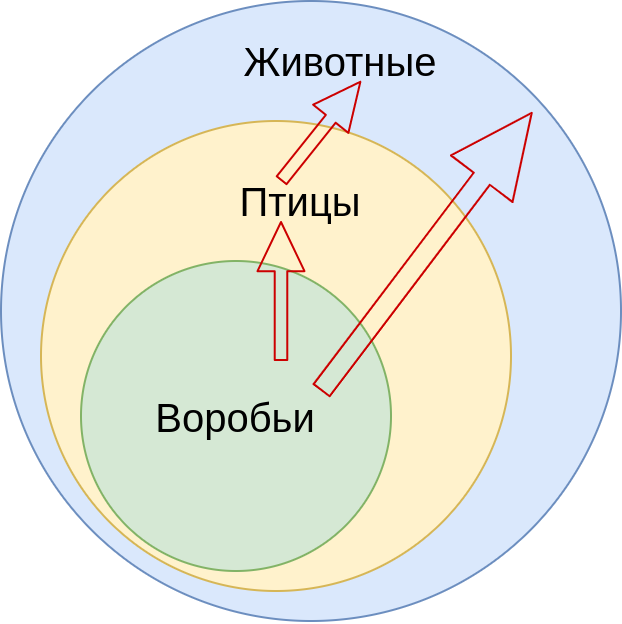
\includegraphics[scale=0.2]{piaf.png}
\end{tabular}
\item При построении суждения посылки могут быть ложными. Более того, в математической логике из ложной посылки следует все, что угодно. Например, \textit{если снег черный, то лес зеленый}. Лес при этом может быть зеленым (летом) и не быть таковым (зимой), но суждение остается истинным, т.к. посылка про снег является ложной.
\item Сравните: если запись числа $a$ оканчивается на 0, то оно кратно 5. Здесь мы ничего не знаем про число $a$, но если для него выполняется посылка, то выполняется и вывод. А если не выполняется, то истинность самого сужджения при этом никак не страдает. Более того, мы знаем, что на 5 также делятся и другие числа, и это значит, что путать местами посылки и вывод ни в коем случае нельзя! Ведь \textbf{не всегда верно}, что если число делится на 5, то его запись заканчивается на 0.
\item Другой~пример:\nopagebreak

\begin{tabular}{lr}
\begin{minipage}[b]{0.5\linewidth}
(\textit{Некоторые французы --- блондины}) и (\textit{некоторые ученики --- французы}), следовательно, (\textit{некоторые ученики --- блондины}). \textbf{Такое суждение неверно}. Поскольку слово <<некоторые>> не гарантирует, что таковым признаком обладают все французы. А значит, из свойства <<быть французом>> не всегда следует <<быть блондином>>.
\end{minipage}& 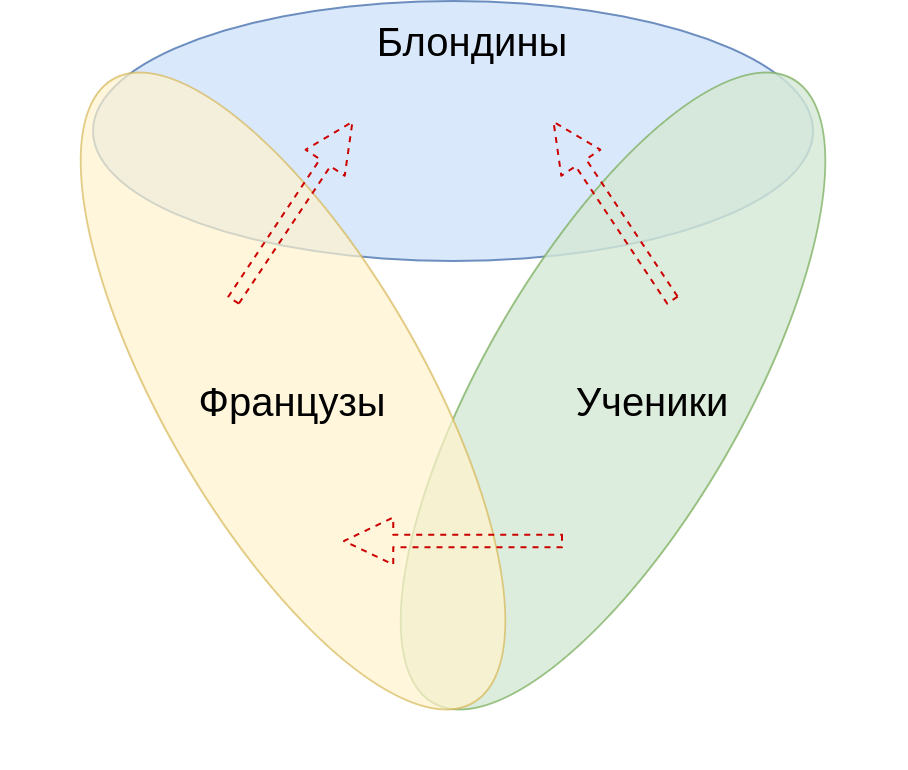
\includegraphics[scale=0.19]{some.png}
\end{tabular}
\item Здесь обе посылки истинные, но вывод ложный. Хотя легко представить ситуацию, когда некоторые ученики действительно будут блондинами. Но это --- лишь предположение, а не строгое рассуждение.
\item В этом примере нарушается именно связка между посылками и выводом, т.к. две посылки не склеиваются по общему признаку. В первой посылке стоит <<некоторые французы>>, а во второй просто <<французы>>, это разные \textbf{множества}, а потому связать две посылки вместе мы не можем!
\item Для построения \textbf{силлогизма} принципиально, чтобы связующее звено было одинаковым:

\begin{center}
\textbf{если} ($A$ есть $B$) и ($B$ есть $C$), \textbf{то} ($A$ есть $C$)
\end{center}
здесь связывание посылок происходит по свойству $B$, и если в нем допустить какое-то искажение, то можно придти к неверным выводам!
\end{enumerate}
\subsection*{Задачи}
\begin{enumerate}
\item Постройте вывод из посылок: (Сократ человек) И (все люди смертны).
\end{enumerate}


\section{Высказывания и предикаты}

\subsection*{Конспект}
\begin{enumerate}\setlength{\itemsep}{1pt}
\item \textbf{Высказывание} --- это любое утверждение на любом языке, которое может быть либо только истинным, либо только ложным.
\item Примеры высказываний: <<\textit{Шесть больше трех}>>, <<\textit{Дважды два --- пять}>>, <<$\sqrt 2$ --- \textit{число иррациональное}>>, <<\textit{среди натуральных чисел существует наибольшее}>>, <<\textit{всякое четное число является суммой двух простых чисел}>>.
\item Все эти высказывания имеют либо истинное, либо ложное значение, хотя про последнее мы не знаем точный ответ. Но мы точно знаем, что их значения не могут быть переменными, т.е. зависеть от каких-то внешних факторов или других высказываний.
\item Из выше приведенных примеров: <<\textit{все птицы --- животные}>> и <<\textit{все воробьи --- птицы}>> есть истинные высказывания.
\item Но эти высказывания можно разобрать на составляющие. Для чего нам понадобятся предикаты.
\item \textbf{Предикат} --- это суждение, зависящее от переменных, обозначающих объекты данного суждения.
\item Например, <<$x$ \textit{есть воробей}>>, <<$x$ \textit{есть птица}>>, <<$x$ \textit{есть животное}>>. Каждое из них может быть истииным или ложным, смотря что подставить вместо $x$. При $x=$ <<\textit{рыба}>> первые два будут ложными, а при $x=$ <<\textit{ромашка}>> ложными будут все три предиката.
\item Аналогично, <<$x$ \textit{есть ученик}>>, <<$x$ \textit{есть француз}>>, <<$x$ \textit{есть блондин}>>. Заметим, что если ранее мы оперировали \textbf{свойствами} (быть учеником, французом, блондином), то теперь перешли к оперированию \textbf{объектом} $x$, который может обладать тем или иным свойством.
\item Из предикатов можно построить новые предикаты, используя логические связки: И($\land$), ИЛИ($\lor$), НЕ($\neg$), СЛЕДУЕТ($\to$).
\item Например, <<($x$ \textit{есть воробей})$\to$($x$ \textit{есть птица}>>), <<($x$ \textit{есть птица})$\to$($x$ \textit{есть животное}>>). Эти предикаты содержат переменную $x$, но они всегда истинны. Такие тождественно истинные предикаты называются \textbf{тавтологиями}. Тавтологии отличаются от истинных высказываний тем, что содержат переменные, которые можно считать фиктивными. Чтобы тавтологию сделать высказыванием, достаточно перед ним сказать <<\textit{для любого} $x$>>, тогда $x$ перестанет быть параметром, а выражение превратится в истинное высказывание:

\begin{center}
<<(\textit{для любого} $x$) ($x$ \textit{есть воробей})$\to$($x$ \textit{есть птица})>>
\end{center}
\item Это называется правилом введения \textbf{квантора всеобщности}.
\item Далее, рассмотрим высказывание <<\textit{некоторые французы блондины}>>. Поступить аналогично предыдущему и заменить его на  предикат <<($x$ \textit{есть француз})$\to$($x$ \textit{есть блондин})>> нельзя! Дело в том, что высказывание <<\textit{все воробьи --- птицы}>> говорит о вложении одного свойства в другое: быть воробьем означает также быть птицей. Но при слове <<\textit{некоторые}>> мы понимаем, что речь идет не о свойстве <<\textit{быть французом}>>, а о том, что некоторые из французов обладают свойством <<\textit{быть блондином}>>. То есть, мы утверждаем, что существует хотя бы один такой объект $x$, который есть и француз и блондин одновременно!
\item Иначе говоря, мы имеем дело со связкой И:
\begin{center}
($x$ \textit{есть француз})$\land$($x$ \textit{есть блондин}),
\end{center}
данный предикат не всегда является истиной, его истинность зависит от конкретного $x$.
\item Тем не менее, и такой предикат можно превратить в высказывание, причем истинное. Для этого нужно слово <<некоторые>> превратить в <<\textit{существует} $x$>>, так что получится истинное высказывание
\begin{center}
<<(\textit{существует} $x$) ($x$ \textit{есть француз})$\land$($x$ \textit{есть блондин})>>
\end{center}
\item Это называется правилом введения \textbf{квантора существования}.
\item Примеры перевода высказываний с языка свойств на язык объектов:\hfill\;

\begin{tabular}{p{0.4\linewidth}p{0.5\linewidth}}\hline
\textit{Все птицы --- животные}  & (\textit{для любого} $x$) ($x$ \textit{есть птица})$\to$($x$ \textit{есть животное}) \\\hline
\textit{Все воробьи --- птицы}  & (\textit{для любого} $x$) ($x$ \textit{есть воробей})$\to$($x$ \textit{есть птица}) \\\hline
\textit{Все воробьи --- животные}  & (\textit{для любого} $x$) ($x$ \textit{есть воробей})$\to$($x$ \textit{есть животное}) \\\hline
Если число заканчивается на 0, то оно кратно 5 &
(\textit{для любого} $a$) ($a$ \textit{заканчивается на $0$})$\to$($a$ \textit{кратно $5$}) \\\hline
Некоторые французы --- блондины 
& (\textit{существует} $x$) ($x$ \textit{есть француз})$\land$($x$ \textit{есть блондин}) \\\hline
Некоторые ученики --- французы 
& (\textit{существует} $x$) ($x$ \textit{есть ученик})$\land$($x$ \textit{есть француз}) \\\hline
Некоторые ученики --- блондины 
& (\textit{существует} $x$) ($x$ \textit{есть ученик})$\land$($x$ \textit{есть блондин}) \\\hline
\end{tabular}

\item Видим, что построить вывод можно только в том случае, когда две посылки склеиваются по общему предикату <<$x$\textit{ есть птица}>>, при этом сами посылки являются импликациями (следование).
\item Можно комбинировать общие и частные суждения:
\begin{center}
<<($x$ \textit{есть птица})$\land$(\textit{все птицы --- животные})>>,
\end{center}
откуда следует вывод <<($x$ \textit{есть животное})>>.

Здесь мы объединили в посылке предикат, что-то говорящий о свойстве объекта $x$, с высказыванием, которое что-то говорит о связи двух свойств, и нашли новое свойство объекта $x$. Это типичное рассуждение от общего к частному.
\item Построение выводов из заданных или полученных ранее истинных высказываний и предикатов называется \textbf{дедукцией} и является основным методом рассуждений при получении математических теорем.
\item Иногда для построения нужного вывода требуетя перебрать сотни комбинаций ранее доказанных посылок. Но часто для нащупывания правильной цепочки доказательства хватает вспомогательных иллюстраций или опыта исследователя, погруженного в данную тему.
\item Ранее мы отмечали, что рассуждения в обратную сторону --- от вывода к посылкам --- неверны. Однако очень часто это верно отчасти. Например, мы знаем дедуктивный вывод: если число оканчивается на 0, то оно делится на 5. На основе этого мы не можем доказать точно, но \textbf{можем предположить}, что если число делится на 5, то оно, вероятно, может оканчиваться на 0. Как мы знаем, это верно примерно в половине случаев. Если бы такое \textit{разворачивание импликации} было бы всегда абсолютно невозможным, то дедукция представляла бы собой простейший случай вывода, когда ложь влечет любое суждение. Для построения теорий это абсолютно бесполезно.
\item Метод \textit{рассуждения назад}, к уже известной посылке, называется \textbf{абдукцией}. Именно таким методом, как правило, пользовался Шерлок Холмс в своих умозаключениях. Именно поэтому его выводы всегда носят вероятностный характер и сопровождаются словами <<вероятно>>, <<скорее всего>> и т.п. Искусство Шерлока Холмса заключается в том, чтобы из всех возможных посылок в данной конкретной ситуации выбрать наиболее вероятную.
\item Например, цитируем из рассказа <<Этюд в багровых тонах>> (Конан Дойль),

\textit{<<Этот человек по типу --- врач, но выправка у него военная. Значит, военный врач. Он только что приехал из тропиков --- лицо у него смуглое, но это не природный оттенок его кожи, так как запястья у него гораздо белее. Лицо изможденное, --- очевидно, немало натерпелся и перенес болезнь. Был ранен в левую руку --- держит ее неподвижно и немножко неестественно. Где же под тропиками военный врач-англичанин мог натерпеться лишений и получить рану? Конечно же, в Афганистане>>. Весь ход мыслей не занял и секунды. И вот я сказал, что вы приехали из Афганистана.}

\item Рассмотрим только часть умозаключений Холмса и сравним их с арифметическим примером\hfill\;

\begin{tabular}{p{0.55\linewidth}p{0.4\linewidth}}\hline
Ватсон --- военный врач с изможденным лицом и загорелый & 
Число 30 --- делится на 5 \\
Воевавшие в Афганистане --- военные с изможденным лицом и загорелые &
Оканчивающее на 0 число --- делится на 5 \\\hline

Вывод: Ватсон прибыл из Афганистана & Вывод: 30 оканчивается на 0\\\hline
\end{tabular}

\item Как видим, нам дано две посылки, в одной из которых дается некая связь между свойствами (воевашие есть военные и т.д., а также оканчивающиеся на 0 делятся на 5), а в другой дается свойство конкретного объекта (Ватсон и число 30). Это свойство общее в обеих посылках, но по нему нельзя склеить их в силлогизм, т.к. свойство всегда стоит в конце посылки. Но Холмс знает, что практически все военные с изможденным лицом и загорелые --- это воевашие в Афганистане (хотя это и неверно на 100\%), и на основании этого он предполагает(!), что и Ватсон такой же, раз он обладает таким же свойством.

\item На примере числа 30 это тоже сработало, однако стоит нам подставить 25 вместо 30, как вся цепочка рассуждений порушится! Поэтому абдуктивные умозаключения нельзя считать математическими, однако они могут навести на правильное дедуктивное умозаключение, в результате чего либо появляется теорема (\textit{Все военные с изможденным лицом воеали в Афганистане}), либо обнаруживается контрпример (в нашем случае это число 25, которое опровергает предположение о том, что все делящиеся на 5 числа оканчаиваются на 0).
\end{enumerate}

\subsection*{Задачи}
\begin{enumerate}
\item Какое абдуктивное предположение можно сделать из следующих посылок: (Зимой выпадает снег) И (Сейчас есть снег) ?
\end{enumerate}


\section{Связь предикатов и множеств}

\subsection*{Конспект}
\begin{enumerate}
\item Выше мы оперировали такими понятиями как свойство и объект, обладающий свойством, на основе чего вводили различные высказывания и предикаты. Посмотрим, как они связаны с понятием \textbf{множество}.
\item Пусть $M$ --- множество всех людей, живущих на планете. Тогда предикат $h(x)$ <<$x$ есть человек>> можно переписать следующим способом: $h(x)=(x\in M)$. Это одновременно означает и то, что $x$ находится в множестве $M$, и то, что $x$ обладает свойством <<быть человеком>>. Говорят также, что $M$ есть область истинности предиката $h(x)$. Таким образом, множество олицетворяет собой свойство, а элементы множества --- объекты, обладающие данным свойством.
\item Если множество $X$ является частью множества $Y$, (например, множество всех женщин есть часть множества $M$), то мы пишем $X\subseteq Y$ ($X$ \textit{содержится в} $Y$, $Y$ \textit{включает} $X$). Важно не путать значки $\in$ и $\subseteq$, т.к. первй говорит о принадлежности объекта к свойству, а второй --- о вложении свойств (о том, что одно свойство меньше или равно другому). Используется также символ строгого вложения $\subset$, означающий, что вложение имеется, но при этом множества не равны.
\item Вложение множеств выражается с помощью принадлежности:
$$
X\subseteq Y\mbox{ эквивалентно }(\forall x) (x\in X)\to(x\in Y)
$$
По сути, это ровно то же самое, что мы ранее делали при переводе языка свойств на язык объектов: \textit{все $X$ есть $Y$} равносильно высказыванию (\textit{для любого} $x$) ($x$ \textit{обладает свойством} $X$)$\to$($x$ \textit{обладает свойством} $Y$).
\item Обозначим далее: $p(x)$ предикат <<$x$ \textit{есть воробей}>>, $o(x)$ предикат <<$x$ \textit{есть птица}>>, $a(x)$ предикат <<$x$ \textit{есть животное}>>. Ранее мы получали следующий вывод:
$$
(\forall x) (p(x)\to o(x))\land (\forall x) (o(x)\to a(x))\vdash(\forall x) (p(x)\to a(x))
$$
\item Попробуем то же самое выразить множествами. Обозначим через $P$ область истинности предиката $p(x)$, т.е. множество всех воробьев, $O$ --- множество всех птиц, $A$ --- множество всех животных. Тогда написанный выше с помощью предикатов вывод можно записать на языке множеств так:
$$
(P\subseteq O\subseteq A) \vdash (P\subseteq A),
$$
поскольку все воробьи есть птицы, все птицы есть животные, а в итоге все воробьи есть животные.
\item На самом деле, существует намного более тесная связь между логическими связками и операциями над множествами.
Вернемся снова к картинке про французов, блондинов и учеников. На ней есть три множества, обозначенные соответствующими овалами. Обозначим их следующим способом:
$$
F = \{x\mid x\mbox{ --- француз}\},\quad B = \{x\mid x\mbox{ --- блондин}\},\quad E = \{x\mid x\mbox{ --- ученик}\}
$$
\item Здесь можно увидеть примеры \textbf{пересечений} множеств:
\begin{gather*}
F\cap B = \{x\mid (x\mbox{ --- француз})\land (x\mbox{ --- блондин})\},\\
F\cap E = \{x\mid (x\mbox{ --- француз})\land (x\mbox{ --- ученик})\},\\
E\cap B = \{x\mid (x\mbox{ --- ученик})\land (x\mbox{ --- блондин})\}.
\end{gather*}
Видим, что они соответствуют логической связке И соответствующих предикатов, выражающих свойства.
\item На той же схеме мы можем усмотреть и такие теоретико-множественные конструкции, как:
$$
F\setminus B = \{x\mid (x\mbox{ --- француз})\land \neg(x\mbox{ --- блондин})\},
$$
т.е. множество французов, не являющихся блондинами. $F\setminus B$ есть операция \textbf{вычитания} множеств.
\item Наконец, множество 
$$
F\cup E  = \{x\mid (x\mbox{ --- француз})\lor (x\mbox{ --- ученик})\}
$$
представляет собой свойство быть французом ИЛИ учеником. Оно содержит в себе как всех французов, так и всех учеников, причем среди них есть как французы, не являющиеся учениками, так и французы, являющиеся уничениками, а также ученики, не являющиеся французами. \textbf{Объединение} множеств соответствует логической связке ИЛИ.
\item Итак, мы можем легко оперировать предикатами, представляя, что они выражают свойство объекта принадлежать некоторому множеству, и наоборот, оперировать множествами, представляя, что оперируем предикатами, для которых эти множества суть область истинности. При этом И соответствует пересечению, ИЛИ --- обединению множеств. Отрицание соответствует вычитанию множеств, причем разность $X\setminus Y$ можно рассматривать как пересечение $X\cap(\neg Y)$. Наконец, вложение множеств соответствует импликации предикатов.
\end{enumerate}



\subsection*{Задачи}
\begin{enumerate}
\item Выразить свойство <<\textit{быть учеником и блондином одновременно}>> через множества $E$ и $B$.
\item Написать множество, соответствующее всем <<\textit{птицам, не являющимся воробьями}>> через множества $O$ и $P$.
\item Какие элементы содержит множество $P\setminus A$, множество $M\cap F$, множество $(F\cup B)\setminus (F\cap B)$?
\item Что выражает высказывание $(M\setminus F)\subseteq (M\setminus B)$?
\item Докажите: $(E\subseteq F)\vdash (M\setminus F)\subseteq (M\setminus E)$ (от противного).
\end{enumerate}


\section{Построение множеств}

\subsection*{Конспект}
\begin{enumerate}
\item Построение множеств прямо наследует из их связи с предикатами. Тем не менее, важно знать язык, позволяющмй компактно и наглядно записывать конструктивные примеры построения множеств.
\item Конечное множество, элементами которого являются объекты $a,b,\dots,z$ (их не обязательно 26, просто какой-то набор), обозначается
$$
\{a,b,\dots,z\},
$$
при этом неважно, в каком порядке записаны элементы внутри скобок, и есть ли там дубликаты. Если в списке один и тот же элемент повторяется несколько раз, то его дубли можно спокойно выбрасывать.\footnote{В математике существует понятие \textbf{мультимножество}, в котором как раз количество дубликатов имеет значение и называется кратностью элемента. Мультимножество удобно, например, для записи разложения числа по степеням простых.}
\item Примеры: $\{0\}$, $\{0,1\}$, $\{0,1,2,3\}$, $\{0,0,1,1,1\}$. Последнее множество равно множеству $\{0,1\}$ (убрали кратные вхождения). Еще пример: $\{\}$ --- \textbf{пустое множество}, обозначаемое также символом $\emptyset$.
\item Как мы уже видели ранее, множество можно задать в \textbf{предикативной форме}, общий вид которой такой:
$$
\{x\mid \ph(x)\},\quad \{f(x)\mid \ph(x)\},
$$
где $\ph(x)$ --- это предикат, выражающий свойство объекта $x$, а $f(x)$ --- некоторое преобразование объекта $x$ (функция). 

В первом случае даное множество является областью истинности предиката $\ph(x)$ и содержит в себе все элементы, и только их, для которых $\ph(x)$ истинно. Во втором случае множество содержит все значения функции $f(x)$, примененные к объектам из области истинности $\ph(x)$. Очевидно, что
$$
\{f(x)\mid \ph(x)\} = \{y\mid(y=f(x))\land\ph(x)\}
$$

\item Конечное множество в предикативной форме записывается так:
$$
\{a,b,\dots,z\} = \{x\mid (x=a)\lor(x=b)\lor\dots\lor(x=z)\},
$$
где предикат $\ph(x)=(x=a)\lor(x=b)\lor\dots\lor(x=z)$ выражает свойство $x$ входить в список объектов $a,b,\dots,z$.
\item Объединение (или сумма) множеств:
$$
A\cup B = \{x\mid (x\in A)\lor(x\in B)\},
$$
например, $\{a,b\}\cup\{b,c\}=\{a,b,c\}$.
\item Пересечение множеств:
$$
A\cap B = \{x\mid (x\in A)\land(x\in B)\},
$$
например, $\{a,b\}\cup\{b,c\}=\{b\}$.
\item Разность множеств:
$$
A\setminus B = \{x\mid (x\in A)\land(x\notin B)\},
$$
например, $\{a,b\}\setminus\{b,c\}=\{a\}$. Заметим, что $A\setminus B$ не всегда равно $B\setminus A$.
\item Если элементы множеств --- это числа, то с ними можно производить арифметические операции:
$$
A+B = \{x+y\mid (x\in A)\land(y\in B)\}, \quad kA = \{kx\mid x\in A\},
$$
здесь первое множество --- это сумма по Минковскому двух множеств, оно содержит все возможные суммы $x+y$, где первое слагаемое берется из первого множества, второе --- из второго.

Легко видеть также, что $A+\emptyset=\emptyset$, т.к. предикат $y\in B$ в случае $B=\emptyset$ тождественно ложный.

\textbf{Важно}: не следует путать $A+A$ и $2A$! Например,
$$
\{0,1\}+\{0,1\}=\{0,1,2\},\mbox{ но }2\{0,1\}=\{0,2\}.
$$

\item Аналогично можно определить произведение множеств по Минковскому:
$$
AB = \{xy\mid (x\in A)\land(y\in B)\},
$$
откуда легко определяется степень множества $A^k$, а также его экспонента $\exp(A)=\sum_k(1/k!)A^k$.

Аналогично сумме видим, что $A\emptyset=\emptyset$.
\end{enumerate}





\subsection*{Задачи}
\begin{enumerate}
\item Найти объединение, пересечение и разность множеств $\{0,1,2,3\}$ и $\{1,2,5\}$ (разность как в прямом, так и в обратном порядке).
\item Записать множество $\{0,1,2\}$ в предикативной форме.
\item Записать множество всех простых чисел в предикативной форме.
\item Доказать, что $A+\{0\}=A$, $A\cdot\{1\}=A$.
\item ${}^{**}$Когда $A\setminus B=B\setminus A$?
\item ${}^{***}$Доказать, что $\max\exp(\{0,x\}) = e^x$.
\end{enumerate}


\end{comment}